\documentclass[12pt,a4paper]{article}

% --- PACOTES DE FONTE E IDIOMA ---
\usepackage{mathptmx} % Fonte Times New Roman
\usepackage[utf8]{inputenc}
\usepackage[T1]{fontenc}
\usepackage[portuguese]{babel}
\usepackage{booktabs} 
\usepackage{siunitx} 
\usepackage{minted}
\usepackage{listings}
\usepackage{graphicx} 
\usepackage{caption}
\usepackage{multirow} 
\usepackage{hyperref}
\usepackage{verbatim} 
\usepackage[alf]{abntex2cite} % Citações no padrão ABNT (Autor, Ano)

% --- MARGENS E ESPAÇAMENTO ---
\usepackage[top=3cm, bottom=2cm, left=3cm, right=2cm]{geometry} 
\usepackage{setspace}
\onehalfspacing

% --- FORMATAÇÃO DE TÍTULOS E PARÁGRAFOS (ABNT) ---
\usepackage{titlesec}
\titleformat{\section}{\normalfont\fontsize{12}{15}\bfseries\uppercase}{\thesection}{1em}{}
\titleformat{\subsection}{\normalfont\fontsize{12}{15}\bfseries}{\thesubsection}{1em}{}
\titleformat{\subsubsection}{\normalfont\fontsize{12}{15}\itshape}{\thesubsubsection}{1em}{}

\usepackage{indentfirst}
\setlength{\parindent}{1.25cm}

% --- CONFIGURAÇÃO DE LEGENDAS (ABNT) ---
\usepackage[font=small, labelfont=bf, labelsep=endash]{caption}

% --- OUTROS UTILITÁRIOS ---
\usepackage{amsmath}
\usepackage{amssymb}
\usepackage{subcaption}
\usepackage{cleveref}

\crefname{equation}{equação}{equações}
\crefname{figure}{figura}{figuras}
\crefname{table}{tabela}{tabelas}
\crefname{section}{seção}{seções}
\crefname{chapter}{capítulo}{capítulos}
%\crefname{subsection}{subseção}{subseções}
%\crefname{subsubsection}{subsubseção}{subsubseções}
\crefname{listing}{código}{códigos}
\crefname{appendix}{apêndice}{apêndices}
\crefname{enumi}{item}{itens}

% Redefinição das conjunções para o português
\newcommand{\crefpairconjunction}{ e }
\newcommand{\crefmiddleconjunction}{, }
\newcommand{\creflastconjunction}{ e }
\newcommand{\crefrangeconjunction}{ a }

\begin{document}

\begin{titlepage}
    \begin{center}
        \begin{singlespace}
            \small
            
\includegraphics[width=2cm, trim=0 150 0 0, clip]{assets/brasao4_vertical_cor.pdf} \\
            \vspace{2.1mm}
            UNIVERSIDADE FEDERAL DO CEARÁ \\
            \vspace{2.1mm}
            DEPARTAMENTO DE ENGENHARIA DE TELEINFORMÁTICA \\
            \vspace{2.1mm}
            TI0111 - ESTATÍSTICA PARA ENGENHARIA \\
            \vspace{2.1mm}
            SEMESTRE 2026.2 \\
        \end{singlespace}

        \vspace{4cm}
        
        \textsc{\textbf{DAVI SOUSA TREVIA MAGALHAES (554934)}}\\
        \textsc{\textbf{GIOVANNI GABRIEL REMEDY MILAN (578412)}} \\
        \textsc{\textbf{GUSTAVO OLIVEIRA SEABRA (567464)}}
        
        \vspace{4cm}
        
        \textbf{HOMEWORK 1 - ESTATÍSTICA DESCRITIVA} \\
        \textbf{BIKE SHARING DATASET}
        
        \vspace{7cm}
        \begin{singlespace}
            FORTALEZA -- CE \\
            SETEMBRO, 2026
        \end{singlespace}
    \end{center}
\end{titlepage}

\newpage
\tableofcontents
\newpage

\section*{INTRODUÇÃO}\label{sec:introducao}
\addcontentsline{toc}{section}{INTRODUÇÃO}


Como Ross introduz, "in today’s world that in order to learn about something you must first collect data. Statistics is the art of learning from data. It is concerned with the collection of data, its subsequent description, and its analysis, which often leads to the drawing of conclusions" \cite{ross2020}. Nesse sentido a estatísitica descritiva é a ferramenta primeira que permite a compreensão dos dados coletados, e por consequência dos fenômenos que eles representam, sendo definida como "the way to quantitatively describe/summarise a collection of information" \cite{l01_freq}. Para isso, tabelas e gráficos são "particularly useful ways of presenting data, often revealing important features such as the range, the degree of concentration, and the symmetry of the data" \cite{ross2020}. 

A fim de "revisar e se familizar com os conceitos de estatística descritiva" \cite{hw1_assignment}, o objetivo é aplicar esses conceitos na análise de um sistema de compartilhamento de bicicletas localizado nos Estados Unidos. O conjunto de dados original, \textit{HW1\_bike\_sharing.csv}, contém observações diárias referentes às condições meteorológicas, estações do ano e o volume de usuários do sistema. 

\section{QUESTÃO 1: }\label{sec:questao1}

\section{QUESTÃO 2: }\label{sec:questao2}

\section{QUESTÃO 3: Análise dos dias de menor utilização}\label{sec:questao3}

Nesta questão, investigam-se as condições do clima e da estação do ano associadas aos dias de baixa utilização do sistema a partir da variável \texttt{low\_usage} definida anteriormente (\Cref{sec:questao2}).

\subsection{Utilização do sistema por estação do ano}

A fim de analisar o impacto da sazonalidade no uso do sistema de compatilhamento de bicicletas, a amostra de 300 dias foi agrupada pelas quatro estações do ano (\textit{season}). Para cada subconjunto, extraíram-se o tamanho da amostra ($n$), a média amostral ($\bar{x}$), a mediana ($\tilde{x}$), o desvio padrão amostral ($s$) e a proporção de dias classificados como de baixa utilização ($p_{low}$).

A extração dessas métricas foi realizada computacionalmente por meio da linguagem R, isolando-se os subconjuntos lógicos e aplicando as funções descritivas nativas, conforme ilustrado no \Cref{lst:snippet_season} e os resultados obtidos foram resumidos na \Cref{tab:sazonalidade}.

\begin{listing}[H]
\inputminted[
    firstline=71,
    lastline=76,
    linenos,
    frame=lines,
    framesep=2mm,
    fontsize=\footnotesize,
]{r}{../codigos/Homework_1/question3.R}
\caption{Trecho do script em R para o cálculo descritivo por estação (exemplo da primavera).}
\label{lst:snippet_season}
\end{listing}

\begin{table}[H]
    \centering
    \caption{Indicadores estatísticos do volume de usuários categorizados por estação do ano.}
    \label{tab:sazonalidade}
    \begin{tabular}{lccccc}
        \toprule
        \textbf{Estação} & $\boldsymbol{n}$ & $\boldsymbol{\bar{x}}$ & $\boldsymbol{M_e}$ & $\boldsymbol{s}$ & $\boldsymbol{p_{low}}$ \textbf{(\%)} \\
        \midrule
        1 (Primavera) & 67 & 1682 & 1650 & 579 & 86.57 \\
        2 (Verão)     & 92 & 3775 & 4086 & 1139 & 14.13 \\
        3 (Outono)    & 94 & 4464 & 4616 & 798.3 & 3.19 \\
        4 (Inverno)   & 47 & 4067 & 4187 & 986.1 & 2.13 \\
        \bottomrule
    \end{tabular}
    \vspace{2mm}
    \caption*{\small{\textbf{Nota:} $n$ = tamanho do subgrupo; $\bar{x}$ = média amostral; $M_e$ = mediana; $s$ = desvio padrão amostral; $p$ = proporção de dias ($low\_usage$).}}
\end{table}

Comparando-se os valores da \Cref{tab:sazonalidade}, fica evidente algumas discrepâncias no comportamento dos usuários ao longo das estações. A primavera destaca-se como o período de menor demanda no sistema, registrando uma média de $\bar{x} = 1682$ usuários e uma mediana de $M_e = 1650$, valores inferiores à metade dos observados nas demais estações. Consequentemente, a proporção de dias de baixa utilização na primavera alcança expressivos $86,57\%$, evidenciando uma restrição severa ao uso do serviço neste período.

Em contrapartida, o outono e o inverno exibem os maiores patamares de movimentação, com médias de $\bar{x} = 4464$ e $\bar{x} = 4067$ usuários, respectivamente. Inclusive o outono concentra a maior mediana da amostra ($M_e = 4616$) e a menor incidência de dias de baixa utilização ($p = 3,19\%$). Já o verão, embora apresente um volume substancial de usuários ($\bar{x} = 3775$), manifesta maior dispersão interna ($s = 1139$), o que se reflete em uma faixa interquartil mais ampla.

O \textit{boxplot} (\Cref{fig:boxplot_season}) corrobora os valores da \Cref{tab:sazonalidade}. Nota-se que a caixa da primavera está isolada na base do gráfico, sem sobreposição com as demais distribuições, além de apresentar \textit{outliers} superiores e inferiores. Para as estações de Verão, Outono e Inverno, as medianas posicionam-se em patamares acima de $4000$ usuários. O outono apresenta uma caixa mais compacta, indicando menor dispersão, e \textit{outliers} superiores e inferiores. Enquanto isso, o verão exibe a caixa mais ampla e os maiores \textit{whiskers} sem nenhum \textit{outlier}, refletindo a maior variabilidade interna, e o inverno apresenta uma caixa intermediária, com \textit{outliers} superiores.

\begin{figure}[H]
    \centering
    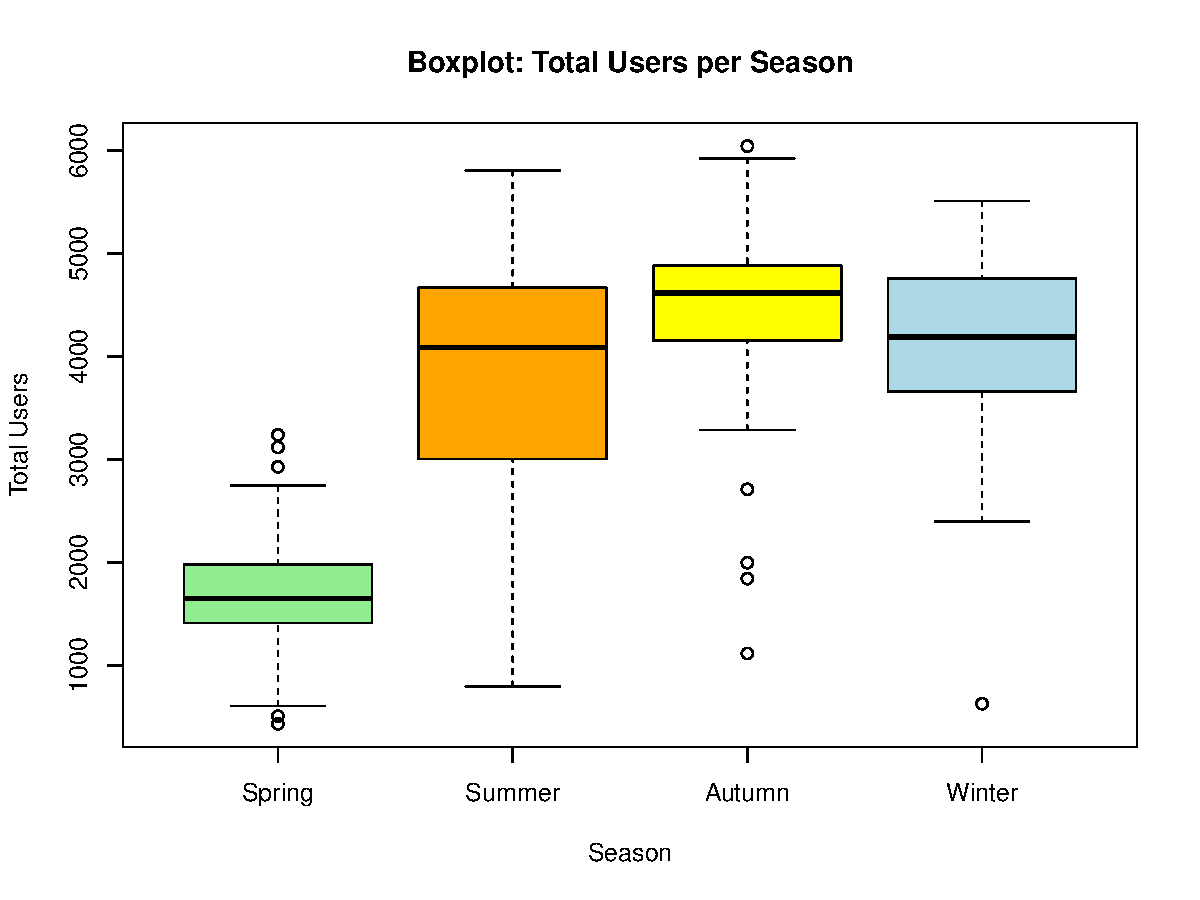
\includegraphics[width=0.8\textwidth]{assets/boxplot_season.pdf}
    \caption{Boxplot comparativo do total de usuários por estação do ano.}
    \label{fig:boxplot_season}
\end{figure} 

Do ponto de vista prático, tais variações demonstram que estações mais secas (como verão, outono e inverno) influenciam diretamente a atratividade do transporte de bicicletas.


\subsection{Utilização do sistema por condições meteorológicas}

Em complemento à análise sazonal, investigou-se a variação no volume de usuários do sistema em função das condições meteorológicas (\textit{weathersit}). Para cada categoria climática registrada na amostra de 300 dias, computaram-se o tamanho do subgrupo ($n$), a média amostral ($\bar{x}$), o desvio padrão amostral ($s$) e a proporção de dias classificados como de baixa utilização ($p_{low}$).

O procedimento computacional para a extração dessas métricas e filtragem das condições de céu limpo, nublado, chuva leve e chuva forteseguiu a mesma lógica de subconjuntos lógicos em R, conforme exemplificado no \Cref{lst:snippet_weather}.

\begin{listing}[H]
\inputminted[
    firstline=215,
    lastline=220,
    linenos,
    frame=lines,
    framesep=2mm,
    fontsize=\footnotesize,
]{r}{../codigos/Homework_1/question3.R}
\caption{Trecho do script em R para o cálculo descritivo por condição meteorológica (exemplo do clima limpo).}
\label{lst:snippet_weather}
\end{listing}

Os resultados estatísticos obtidos para cada condição climática encontram-se resumidos na \Cref{tab:meteorologia}. Destaca-se que a categoria de chuva forte (\textit{Heavy Rain}) não registrou ocorrências no período amostral de 300 dias analisado.

\begin{table}[H]
    \centering
    \caption{Indicadores estatísticos do volume de usuários categorizados por condição meteorológica.}
    \label{tab:meteorologia}
    \begin{tabular}{lcccc}
        \toprule
        \textbf{Condição Meteorológica} & $\boldsymbol{n}$ & $\boldsymbol{\bar{x}}$ & $\boldsymbol{s}$ & $\boldsymbol{p_{low}}$ \textbf{(\%)} \\
        \midrule
        1 (Céu Limpo)        & 186 & 3899   & 1305  & 18.28 \\
        2 (Nublado)         & 104 & 3173   & 1304  & 32.69 \\
        3 (Chuva Fraca) & 10  & 1562   & 851.9 & 70.00 \\
        4 (Chuva Forte) & 0   & --     & --    & --    \\
        \bottomrule
    \end{tabular}
    \vspace{2mm}
    \caption*{\small{\textbf{Nota:} $n$ = tamanho do subgrupo; $\bar{x}$ = média amostral; $s$ = desvio padrão amostral; $p_{low}$ = proporção de dias ($low\_usage$).}}
\end{table}

A análise dos dados evidencia uma forte degradação na atratividade do serviço conforme as condições climáticas se tornam chuvosas. A maior parte dos registros concentra-se sob a condição de céu limpo ($n = 186$ dias), apresentando o maior patamar médio de utilização ($\bar{x} = 3899$ usuários) e a menor incidência de dias de baixa demanda ($p = 18,28\%$).

Sob condições nubladas, observa-se uma redução moderada na média de usuários ($\bar{x} = 3173$), acompanhada por um aumento expressivo na proporção de baixa utilização, que passa a atingir $32,69\%$. No entanto, o impacto mais drástico ocorre em dias de chuva fraca ($n = 10$). Embora representem uma fração minoritária da amostra, a média de usuários desaba para $\bar{x} = 1562$ (menos da metade de um dia limpo), e a proporção de dias classificados como de baixa utilização salta para $70,00\%$.


O \textit{boxplot} (\Cref{fig:boxplot_weather}) corrobora visualmente esses valores. Observa-se que a distribuição do total de usuários sob céu limpo possui sua mediana posicionada no terço superior do gráfico, com a maior amplitude de valores normais e apenas um \textit{outlier} inferior. Conforme o clima transita para a chuva fraca, nota-se um deslocamento progressivo das caixas para patamares inferiores de utilização, acompanhado por uma compressão na dispersão dos dados nos dias chuvosos devido ao baixo volume de operações.

\begin{figure}[H]
    \centering
    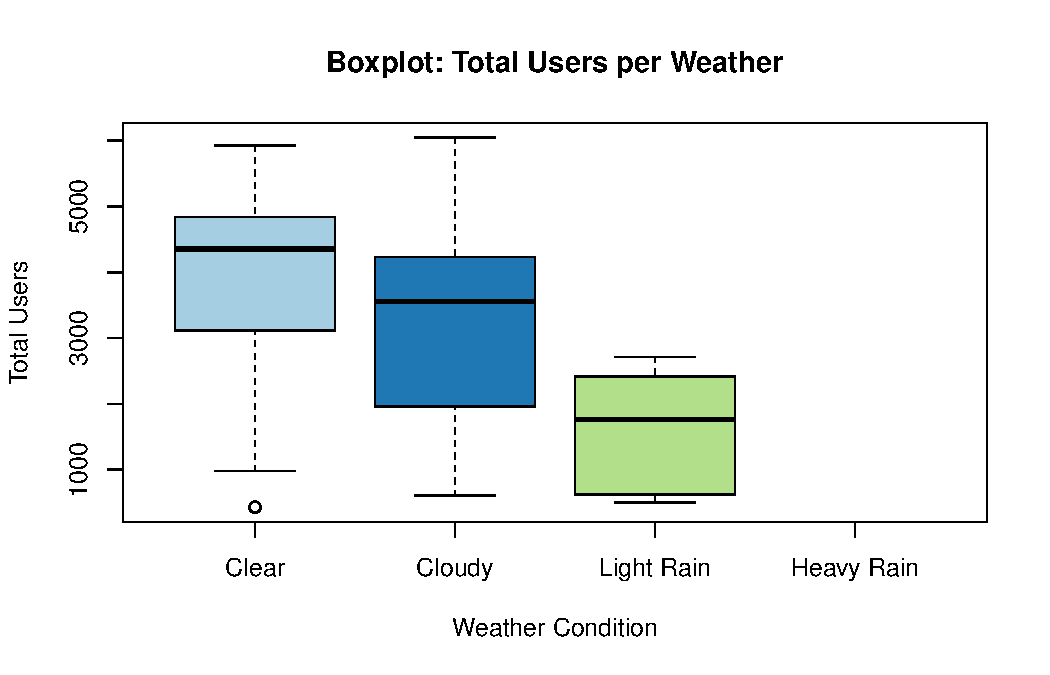
\includegraphics[width=0.8\textwidth]{assets/boxplot_weather.pdf}
    \caption{Boxplot comparativo do total de usuários por condição meteorológica.}
    \label{fig:boxplot_weather}
\end{figure} 

Dessa forma, os dados demonstram que o comportamento aparentemente inesperado observado nas estações do ano (onde períodos de outono e inverno registraram volumes elevados de demanda) encontra sua principal justificativa nas condições meteorológicas. Isso indica que a disposição dos usuários em utilizar o sistema é governada de forma muito mais direta pela presença de precipitação e cobertura de nuvens do que estritamente pela sazonalidade.

\subsection{Relação entre temperatura e utilização diária}

Para investigar a relação entre a temperatura ambiente (\textit{temp}) e o volume diário de locações (\textit{total\_user}), ambas variáveis quantitativas contínuas, adotou-se o Coeficiente de Correlação Amostral de Pearson ($r$). O coeficiente $r$ quantifica a força e a direção da associação linear entre duas variáveis, variando no intervalo $[-1, 1]$ \cite{ross2020}.

Para fins de validação, o cálculo foi primeiramente estruturado de forma manual para as 10 primeiras observações da amostra, computando-se os desvios em relação à média, a soma dos produtos dos desvios (covariância não normalizada) e as somas dos quadrados (variâncias não normalizadas). Posteriormente, o resultado foi confrontado com a função nativa \texttt{cor()} do R. O \Cref{lst:snippet_temp} exibe a implementação deste procedimento.

\begin{listing}[H]
\inputminted[
    firstline=293, 
    lastline=324,
    linenos,
    breaklines,
    breakanywhere,
    frame=lines,
    framesep=2mm,
    fontsize=\footnotesize,
    style=vs
]{r}{../codigos/Homework_1/question3.R}
\caption{Trecho do script em R para o cálculo manual e automatizado da correlação de Pearson.}
\label{lst:snippet_temp}
\end{listing}

A validação no subconjunto de 10 amostras retornou um coeficiente $r \approx 0,4414$. A comparação entre o cálculo desenvolvido passo a passo e o executado pela função interna do R revelou uma diferença residual de $5,551 \times 10^{-17}$. Cumpre ressaltar que esta discrepância pequena não configura um erro metodológico, mas sim um erro de arredondamento inerente à precisão de ponto flutuante da própria linguagem \cite{kerns2010}.

Ao escalar o cálculo para a amostra completa ($n = 300$), obteve-se um coeficiente de correlação $r = 0,7839$. Segundo Ross e os slides da disciplina \cite{ross2020, l04_wrap}, valores de $|r|$ próximos a $0,8$ indicam uma associação linear positiva de intensidade forte. Isso significa que, em termos globais, o aumento da temperatura ambiente está fortemente associado ao aumento no número de bicicletas alugadas.

\begin{figure}[H]
    \centering
    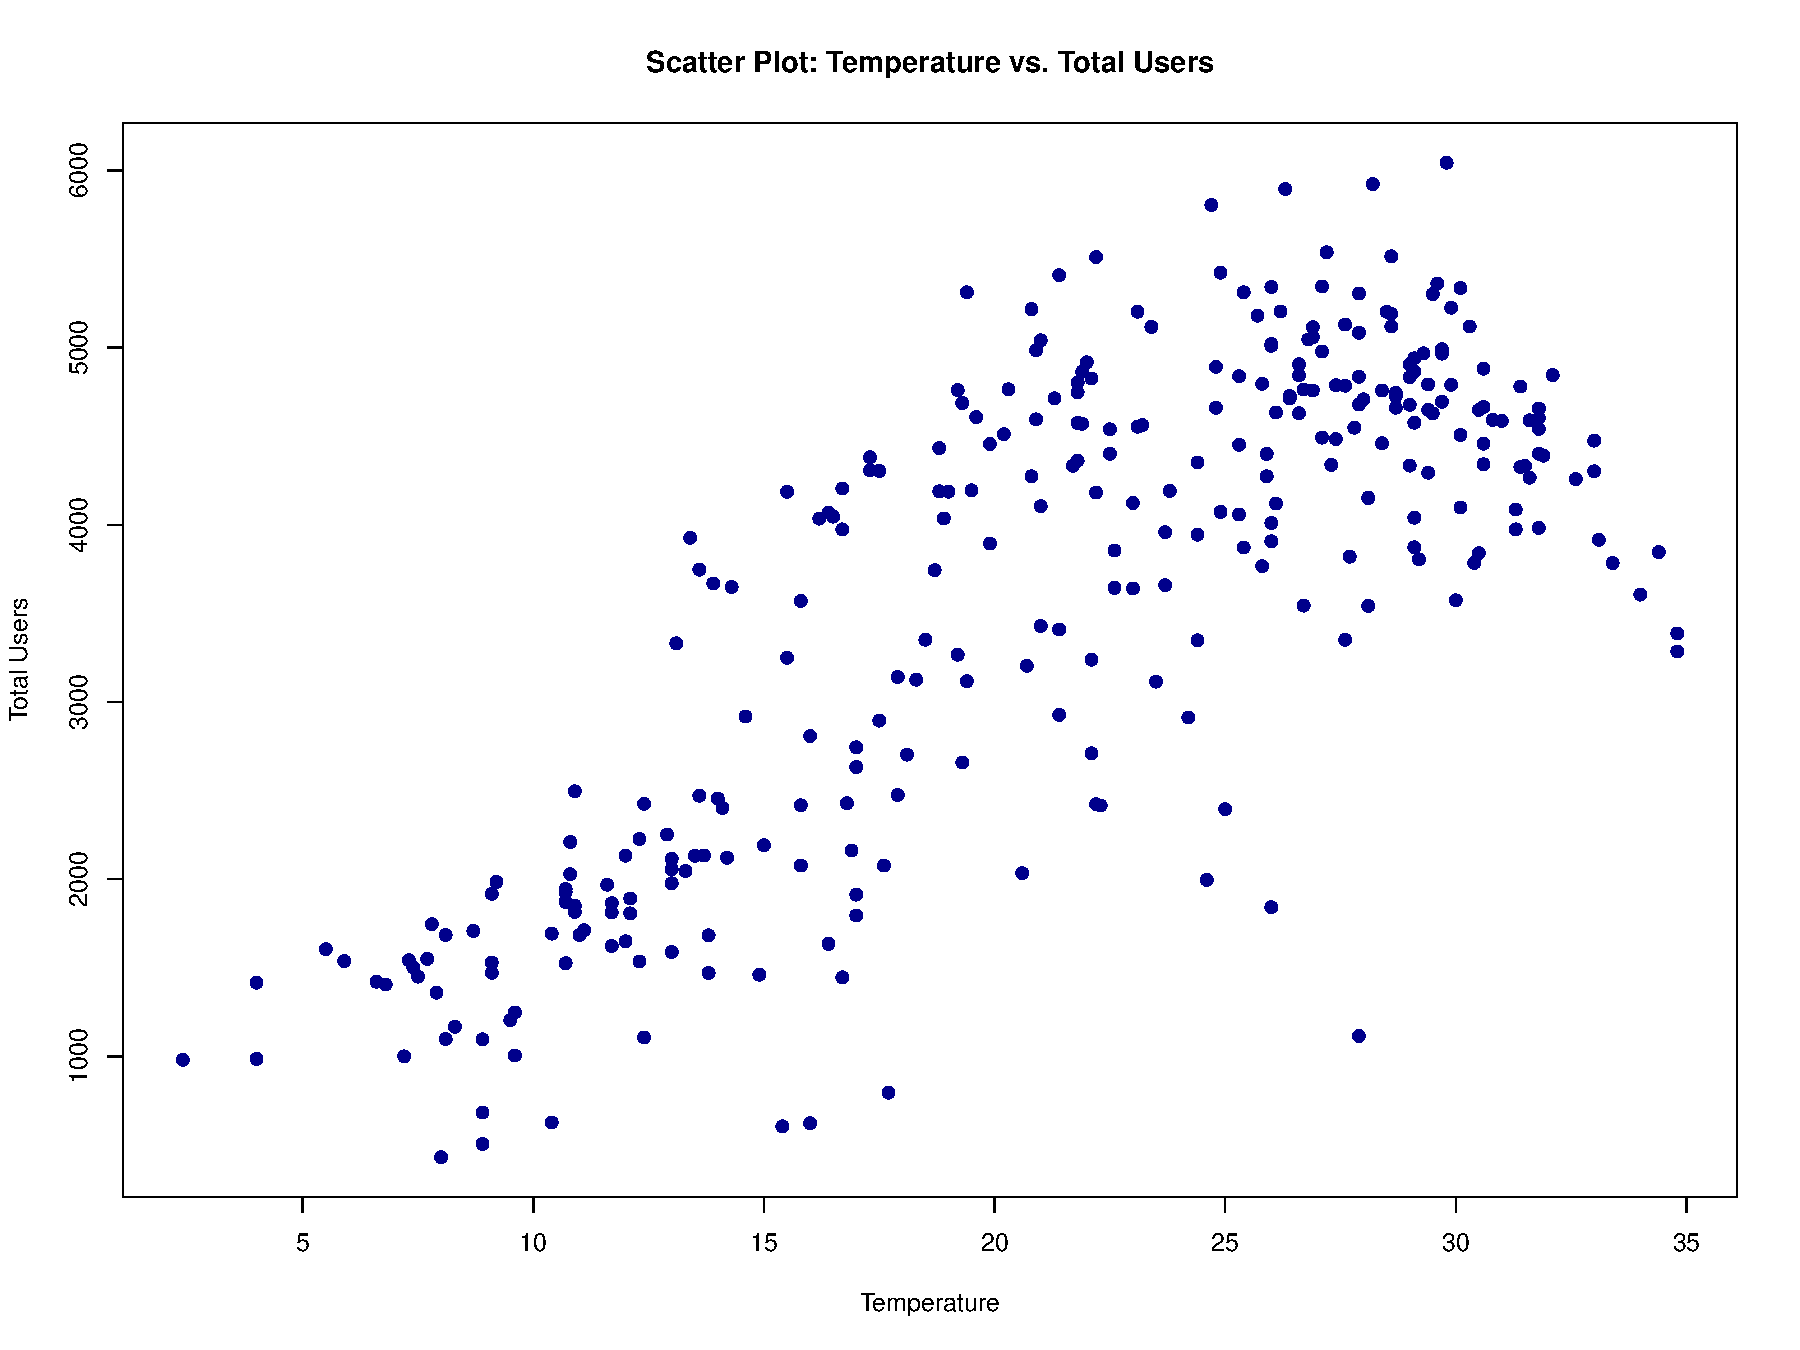
\includegraphics[width=0.85\textwidth]{assets/scatter_temp.pdf}
    \caption{Diagrama de dispersão evidenciando a associação linear positiva entre a temperatura real (°C) e o total de usuários.}
    \label{fig:scatter_temp}
\end{figure}

A análise visual do diagrama de dispersão (\Cref{fig:scatter_temp}) confirma a natureza positiva e proporcional da relação. Observa-se uma nuvem de pontos com clara tendência ascendente à medida que a temperatura avança dos $5^\circ\text{C}$ em direção aos $25^\circ\text{C}$. 

Contudo, a inspeção gráfica também evidencia as limitações da correlação linear estrita: ao atingir temperaturas extremas (próximas ou superiores a $30^\circ\text{C}$), a tendência de crescimento cessa e a nuvem de pontos aparenta estabilizar ou declinar levemente. Tal comportamento sugere a existência de um ponto de saturação de conforto térmico, a partir do qual o calor excessivo passa a desencorajar atividades físicas ao ar livre.

\subsection{Seleção das características mais associadas à utilização}

Com base nas análises exploratórias conduzidas nas subseções anteriores, selecionaram-se a temperatura (\textit{temp}) e as condições meteorológicas (\textit{weathersit}) como as duas características que exercem a maior influência sobre a demanda do sistema de compartilhamento de bicicletas.

A escolha da temperatura justifica-se quantitativamente pelo forte coeficiente de correlação linear positivo ($r = 0,7839$) e pela evidência visual do diagrama de dispersão (\Cref{fig:scatter_temp}), demonstrando que o conforto térmico é um impulsionador contínuo para o uso do sistema. Por sua vez, as condições meteorológicas atuam como um fator restritivo categórico diário: a ocorrência de precipitação deprime drasticamente a média de locações e eleva a probabilidade de baixa utilização para $70\%$, conforme a \Cref{tab:meteorologia}.

Para complementar a dinâmica dessas variáveis, elaborou-se um \textit{boxplot} duplo comparando a distribuição da temperatura em relação à sazonalidade e ao clima (\Cref{fig:boxplots_temp}).

\begin{figure}[H]
    \centering
    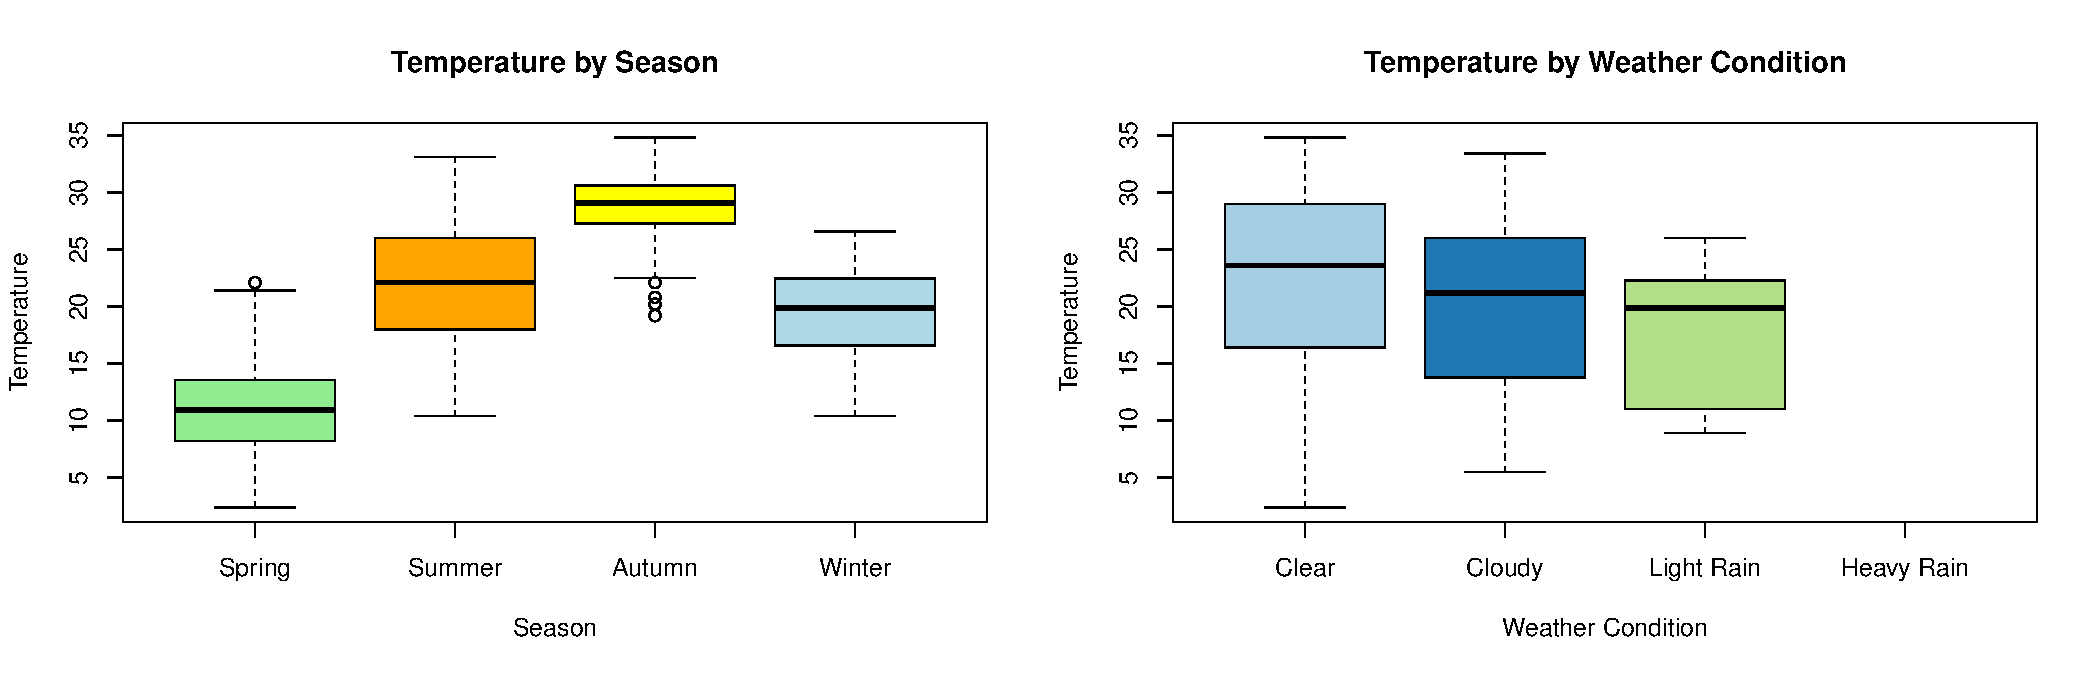
\includegraphics[width=1\textwidth]{assets/boxplots_temp.pdf}
    \caption{Painel comparativo da distribuição de temperatura pelas estações do ano e condições meteorológicas.}
    \label{fig:boxplots_temp}
\end{figure}

A inspeção do painel direito da \Cref{fig:boxplots_temp} revela que as temperaturas máximas apresentam um declínio visível à medida que o clima transita para cenários de chuva. Concomitantemente, o painel esquerdo expõe a forte segmentação térmica imposta pela sazonalidade, onde a primavera concentra as temperaturas mais baixas e o outono as mais altas da amostra analisada. 

Sob a ótica da mobilidade urbana, esses resultados comprovam que a dinâmica do sistema é otimamente modelada pelo par \textit{Temperatura} e \textit{Clima}: a temperatura fornece a escala contínua de atratividade térmica, enquanto o clima atua como um limitador imediato (presença ou ausência de chuva).

\section{QUESTÃO 4: }\label{sec:questao4}

\section*{CONCLUSÃO}\label{sec:conclusao}
\addcontentsline{toc}{section}{CONCLUSÃO}

\newpage
\appendix
\section*{APÊNDICES}\label{sec:apendices}
\addcontentsline{toc}{section}{APÊNDICES}

\section{CÓDIGO FONTE EM R UTILIZADO NAS ANÁLISES}

Os códigos a seguir apresentam o código-fonte completo desenvolvido em R para a execução de todas as etapas estatísticas e gráficas deste relatório disponível no repositório \cite{github_repo}. Os scripts são totalmente funcionais e executáveis, tendo sido desenvolvidos segundo a \Cref{tab:scripts}.

\begin{table}[H]
    \centering
    \caption{Scripts em R utilizados para cada questão do relatório.}
    \label{tab:scripts}
    \begin{tabular}{l | cc}
        \toprule
        \textbf{Membro} & \textbf{Questão} & \textbf{Script em R} \\
        \midrule
        Davi S. T. Magalhães & 1 e 2 & main.R \\
        Giovanni G. R. Milan & 3 & question3.R \\
        Gustavo O. Seabra & 4 & - \\
        \bottomrule
    \end{tabular}
\end{table}

\subsection{Script questões 1 e 2 (main.R)}
\inputminted[
    linenos,
    breaklines,
    breakanywhere,
    frame=lines,
    framesep=2mm,
    fontsize=\scriptsize,
]{r}{../codigos/Homework_1/main.R}


\subsection{Script questão 3 (question3.R)}
\inputminted[
    linenos,
    breaklines,
    breakanywhere,
    frame=lines,
    framesep=2mm,
    fontsize=\scriptsize,
]{r}{../codigos/Homework_1/question3.R}

\begin{comment}
\subsection{Script questão 4 (___.R)}
\inputminted[
    linenos,
    breaklines,
    breakanywhere,
    frame=lines,
    framesep=2mm,
    fontsize=\scriptsize,
]{r}{../codigos/Homework_1/___.R}
\end{comment}

\bibliography{refs}
\end{document}